\section{Issues Encountered So Far}

\subsection{Non Deterministic Nature of the Extraction Algorithm}

The extraction algorithm used by RA is non-deterministic. This means that for a
given code input, the output of the extraction algorithm can vary. It produces
semantically different but functionally identical code. This has been a massive
issue when trying to test the tool, as the output of the tool can vary between
runs, as shown in the below example of a simple function extraction, where the
tool has passed references to the extracted function and then dereferenced the
reference, rather than passing ownership of \textcolor{blue}{\texttt{n}}. Whilst
these are likely to compile to the same assembly, from a readability
perspective, the output is not ideal.

\begin{figure}[H]
    \centering
    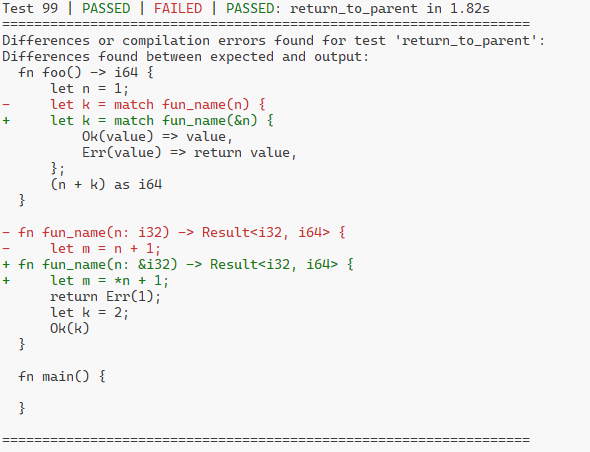
\includegraphics[width=\columnwidth]{Figures/issue_1.png}
    \caption{An example of the non-deterministic nature of the extraction
    algorithm. \textcolor{red}{Red is expected output}, \textcolor{green}{green is the
    returned code}}
    \label{fig:issue1}
\end{figure}